\section{Tools}

\section{Test Data}
For testing purposes a set of prerecorded power data provided by the UK Energy Research Centre Energy Data Centre (UKERC-EDC) is used\cite{ukerc}.
This test set contains various types of data including 16 kHz recorded voltage and current values for a house in the UK, which will be used in the proposed thesis.

In chapter \ref{electric_characteristics} the optimal sample rate for measuring power quality parameters was calculated to be 20 kHz. Although the test data set has a sample rate of only 16 kHz, it can be used for simulation purposes. The slower sample rates result in a loss of information in the upper harmonics which have no big impact on the simulation, especially on the amount of data that has to be transferred from the measurement devices to the cloud system.

The recorded data is provided as flac-files\footnote{Free Lossless Audio Codec\cite{flac}}. Each file contains one hour of recording in a compressed format. The following procedure describes how to decode the values such that they can be used in the simulation environment.

\begin{enumerate}
	\item Convert flac-file to wav-file with sox\cite{sox}: \\ \lstinline[language=bash,basicstyle=\ttfamily]{sox.exe data.flac -e signed-integer -b 32 data.wav}
	\item Decode wav-file according to its specification\cite{wav}:
	\begin{enumerate}
		\item Deocode file header
		\item Decode data section
	\end{enumerate}
\end{enumerate}

The wav-files holds the values for voltage and current as consecutive 32-Bit-Integer values. First value is voltage, second is current and so on. These values has to be multiplied with calibration factors (also provided in the data sets) to get the real values for voltage and current. After this transformation, the values can be used in the simulation. Figure \ref{fig:test_data} shows an excerpt of the data after the transformation.

\begin{figure}[h]
	\centering
		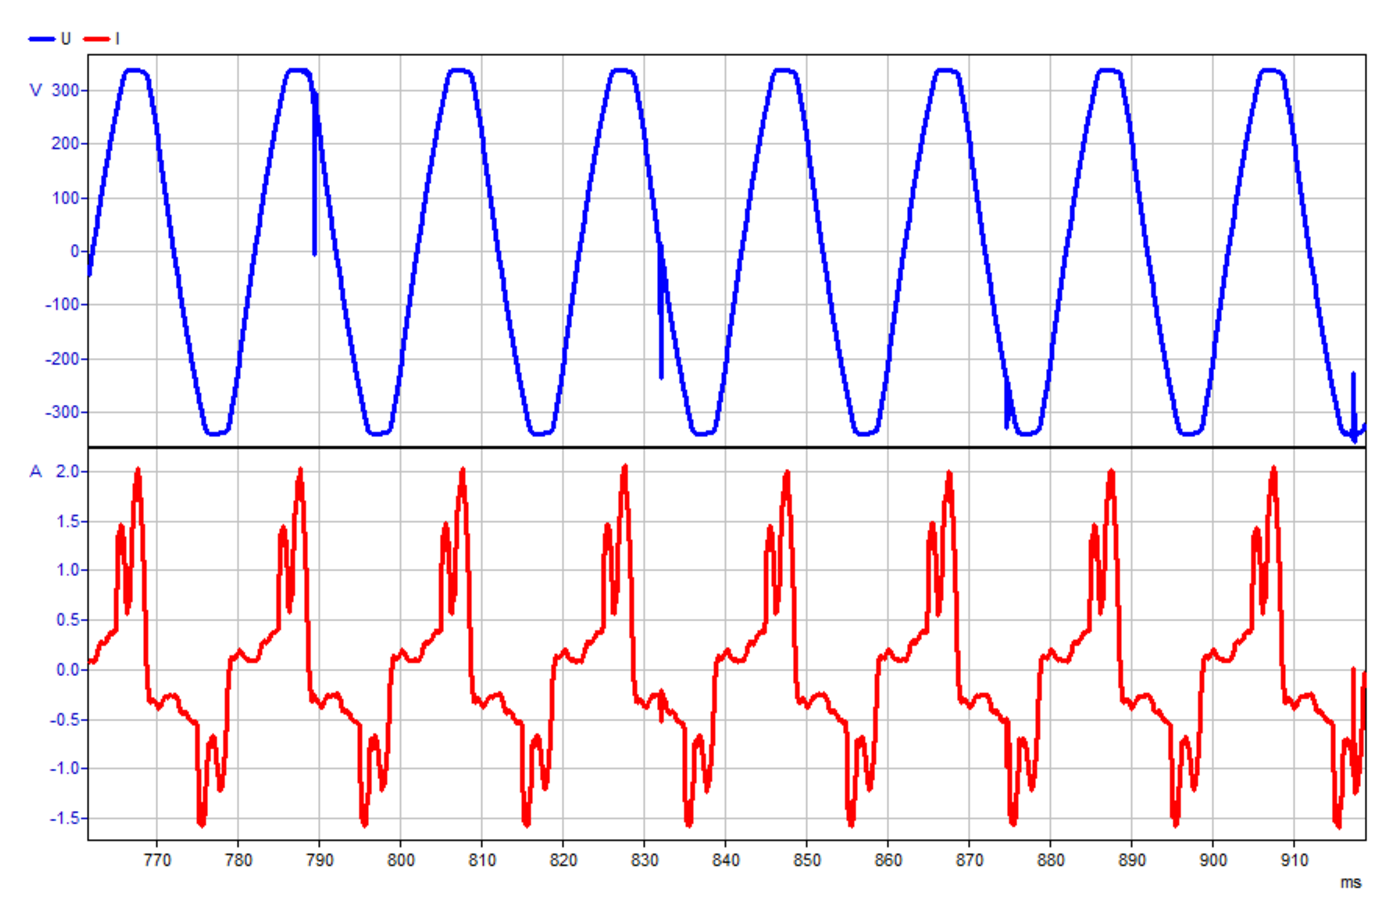
\includegraphics[scale=0.5]{graphics/testdata.eps}
	\caption{Test data}
	\label{fig:test_data}
\end{figure}

\section{Simulation Design}

Figure \ref{fig:simulation_design} shows the general simulation setup that is used to test the software components of the proposed system.

\begin{figure}[h]
	\centering
		\includegraphics[scale=0.7]{graphics/simulation_2.eps}
	\caption{Simulation design}
	\label{fig:simulation_design}
\end{figure}

Different parameters of the simulation can be changed, such that different environments can be simulated and evaluated against each other. The following enumeration describes the parameters that can be adapted as input data to the simulation:

\begin{itemize}
	\item Bandwidth of the Internet connection
		\begin{itemize}
			\item Wired connection: 100 MB/s, 50 MB/s, 20 MB/s, 10 MB/s
			\item WiFi connection: 
			\item Cellphone connection: LTE (), 4G (), 2G (), GPRS ()
		\end{itemize}
	\item Number of PQM meters
	\item Number of Webservices
	\item Transmitted data
		\begin{itemize}
			\item Raw data
			\item Preprocessed data
		\end{itemize}
  \item Storage
		\begin{itemize}
			\item File archive
			\item SQL database (MySQL)
			\item NoSQL database (CrateDB)
		\end{itemize}		
\end{itemize}

Modifications of the above mentioned parameters have an effect to the following parts:

\begin{itemize}
	\item Server side storage
	\item Network load, network costs
	\item Server side throughput
\end{itemize}

Table \ref{tab:SimulationResults} shows the expected results of the simulation:

\begin{table}[h]
\centering
\begin{tabular}{l|c|c|c|c}
\hline
\multicolumn{1}{l|}{\multirow{2}{*}{\textbf{Parameter}}} & \multicolumn{1}{c|}{\multirow{2}{*}{\textbf{Modification}}} & \multicolumn{3}{c}{\textbf{Impact}}                                                                                                  \\ \cline{3-5} 
\multicolumn{1}{c|}{} & \multicolumn{1}{c|}{}  & \multicolumn{1}{c|}{\textbf{Bandwidth}} & \multicolumn{1}{c|}{\textbf{Server storage}} & \multicolumn{1}{c}{\textbf{Throughput}} \\ \hline \hline
\multirow{2}{*}{\textbf{Bandwidth}} & \cellcolor{green} & \cellcolor{green} &\cellcolor{yellow}&\cellcolor{yellow}\\
\cline{2-5} 
                                                         & \cellcolor{red}                                                           & \cellcolor{red}                                       &\cellcolor{yellow}                                                &\cellcolor{yellow}                                      \\ \hline
\multirow{2}{*}{\textbf{Number of PQM meters}}           & \cellcolor{green}                                                           & \cellcolor{green}                                       & \cellcolor{green}                                                 & \cellcolor{red}                                       \\ \cline{2-5} 
                                                         & \cellcolor{red}                                                           & \cellcolor{red}                                       & \cellcolor{red}                                                 & \cellcolor{green}                                       \\ \hline
\multirow{2}{*}{\textbf{Number of web services}}          & \cellcolor{green}                                                           &\cellcolor{yellow}                                      &\cellcolor{yellow}                                                & \cellcolor{green}                                       \\ \cline{2-5} 
                                                         & \cellcolor{red}                                                           &\cellcolor{yellow}                                      &\cellcolor{yellow}                                                & \cellcolor{red}                                       \\ \hline
\multirow{2}{*}{\textbf{Transmitted Data}}               & \cellcolor{green}                                                           & \cellcolor{green}                                       & \cellcolor{green}                                                 & \cellcolor{red}                                       \\ \cline{2-5} 
                                                         & \cellcolor{red}                                                           & \cellcolor{red}                                       & \cellcolor{red}                                                 & \cellcolor{green}                                       \\ \hline
\multirow{3}{*}{\textbf{Server side storage}}            & File                                                        &\cellcolor{yellow}                                      & \cellcolor{purple}                                                 &\cellcolor{yellow}                                      \\ \cline{2-5} 
                                                         & SQL                                                         &\cellcolor{yellow}                                      & \cellcolor{purple}                                                 &\cellcolor{yellow}                                      \\ \cline{2-5} 
                                                         & NoSQL                                                       &\cellcolor{yellow}                                      & \cellcolor{purple}                                                 &\cellcolor{yellow}                                      \\ \hline
\end{tabular}
\caption{Simulation results}
\label{tab:SimulationResults}
\end{table}

\section{Evaluation}

\section{Impact on System Design}